\chapter{Event-Driven Molekulardynamik}

Im Gegensatz zum Ansatz in der vorherigen Arbeit (vgl \cite{eibl2012}), besch�ftigt sich diese Arbeit mit einem anderen Ansatz die Dynamik von Teilchen zu simulieren. Dabei werden nicht die Bewegungsgleichungen der einzelnen Teilchen um einen festen Zeitschritt integriert, um ihre Ortskurven zu erhalten und ihr Verhalten zu bestimmen, sondern die Simulation entwickelt sich von Ereignis zu Ereignis. Ein Ereignis in diesem Zusammenhang kann zum Beispiel eine Teilchen-Teilchen-Kollision, eine Teilchen-Wand-Kollision, ein Aktualisieren des Bildschirms, etc sein. Bei dieser Art der Simulation k�nnen keine kontinuierlichen Teilchenpotentiale mehr betrachtet werden. Stadtessen werden Sprungpotentiale verwendet:
\begin{equation}
V(r) = \left\{ 
\begin{array}{lll} 
\infty & \quad \text{f�r} & r\leq R \\  
0 & \quad\text{f�r} & r>R 
\end{array}
\right.
\end{equation}
wobei $R$ der Radius des Teilchens ist. Dies entspricht einem Harte-Kugel-Fluid, bei dem die Teilchen wie Billardkugeln miteinander sto�en.

Die erste m�gliche Implementation ist nun, alle m�glichen Ereignisse zu berechnen, die Simulation auf den Zeitpunkt des fr�hesten Ereignisses zu setzen und das Ereignis auszuf�hren. Daf�r m�ssen in jedem Schritt die Kollisionen von allen Teilchen mit allen anderen berechnet werden. Dies f�hrt zu einer quadratischen Laufzeit mit der Teilchenzahl (\fref{fig:A1_runtime}). F�r eine ernsthafte Simulation ist diese Variante deswegen unpraktisch.

\begin{figure}[h!]
	\centering
		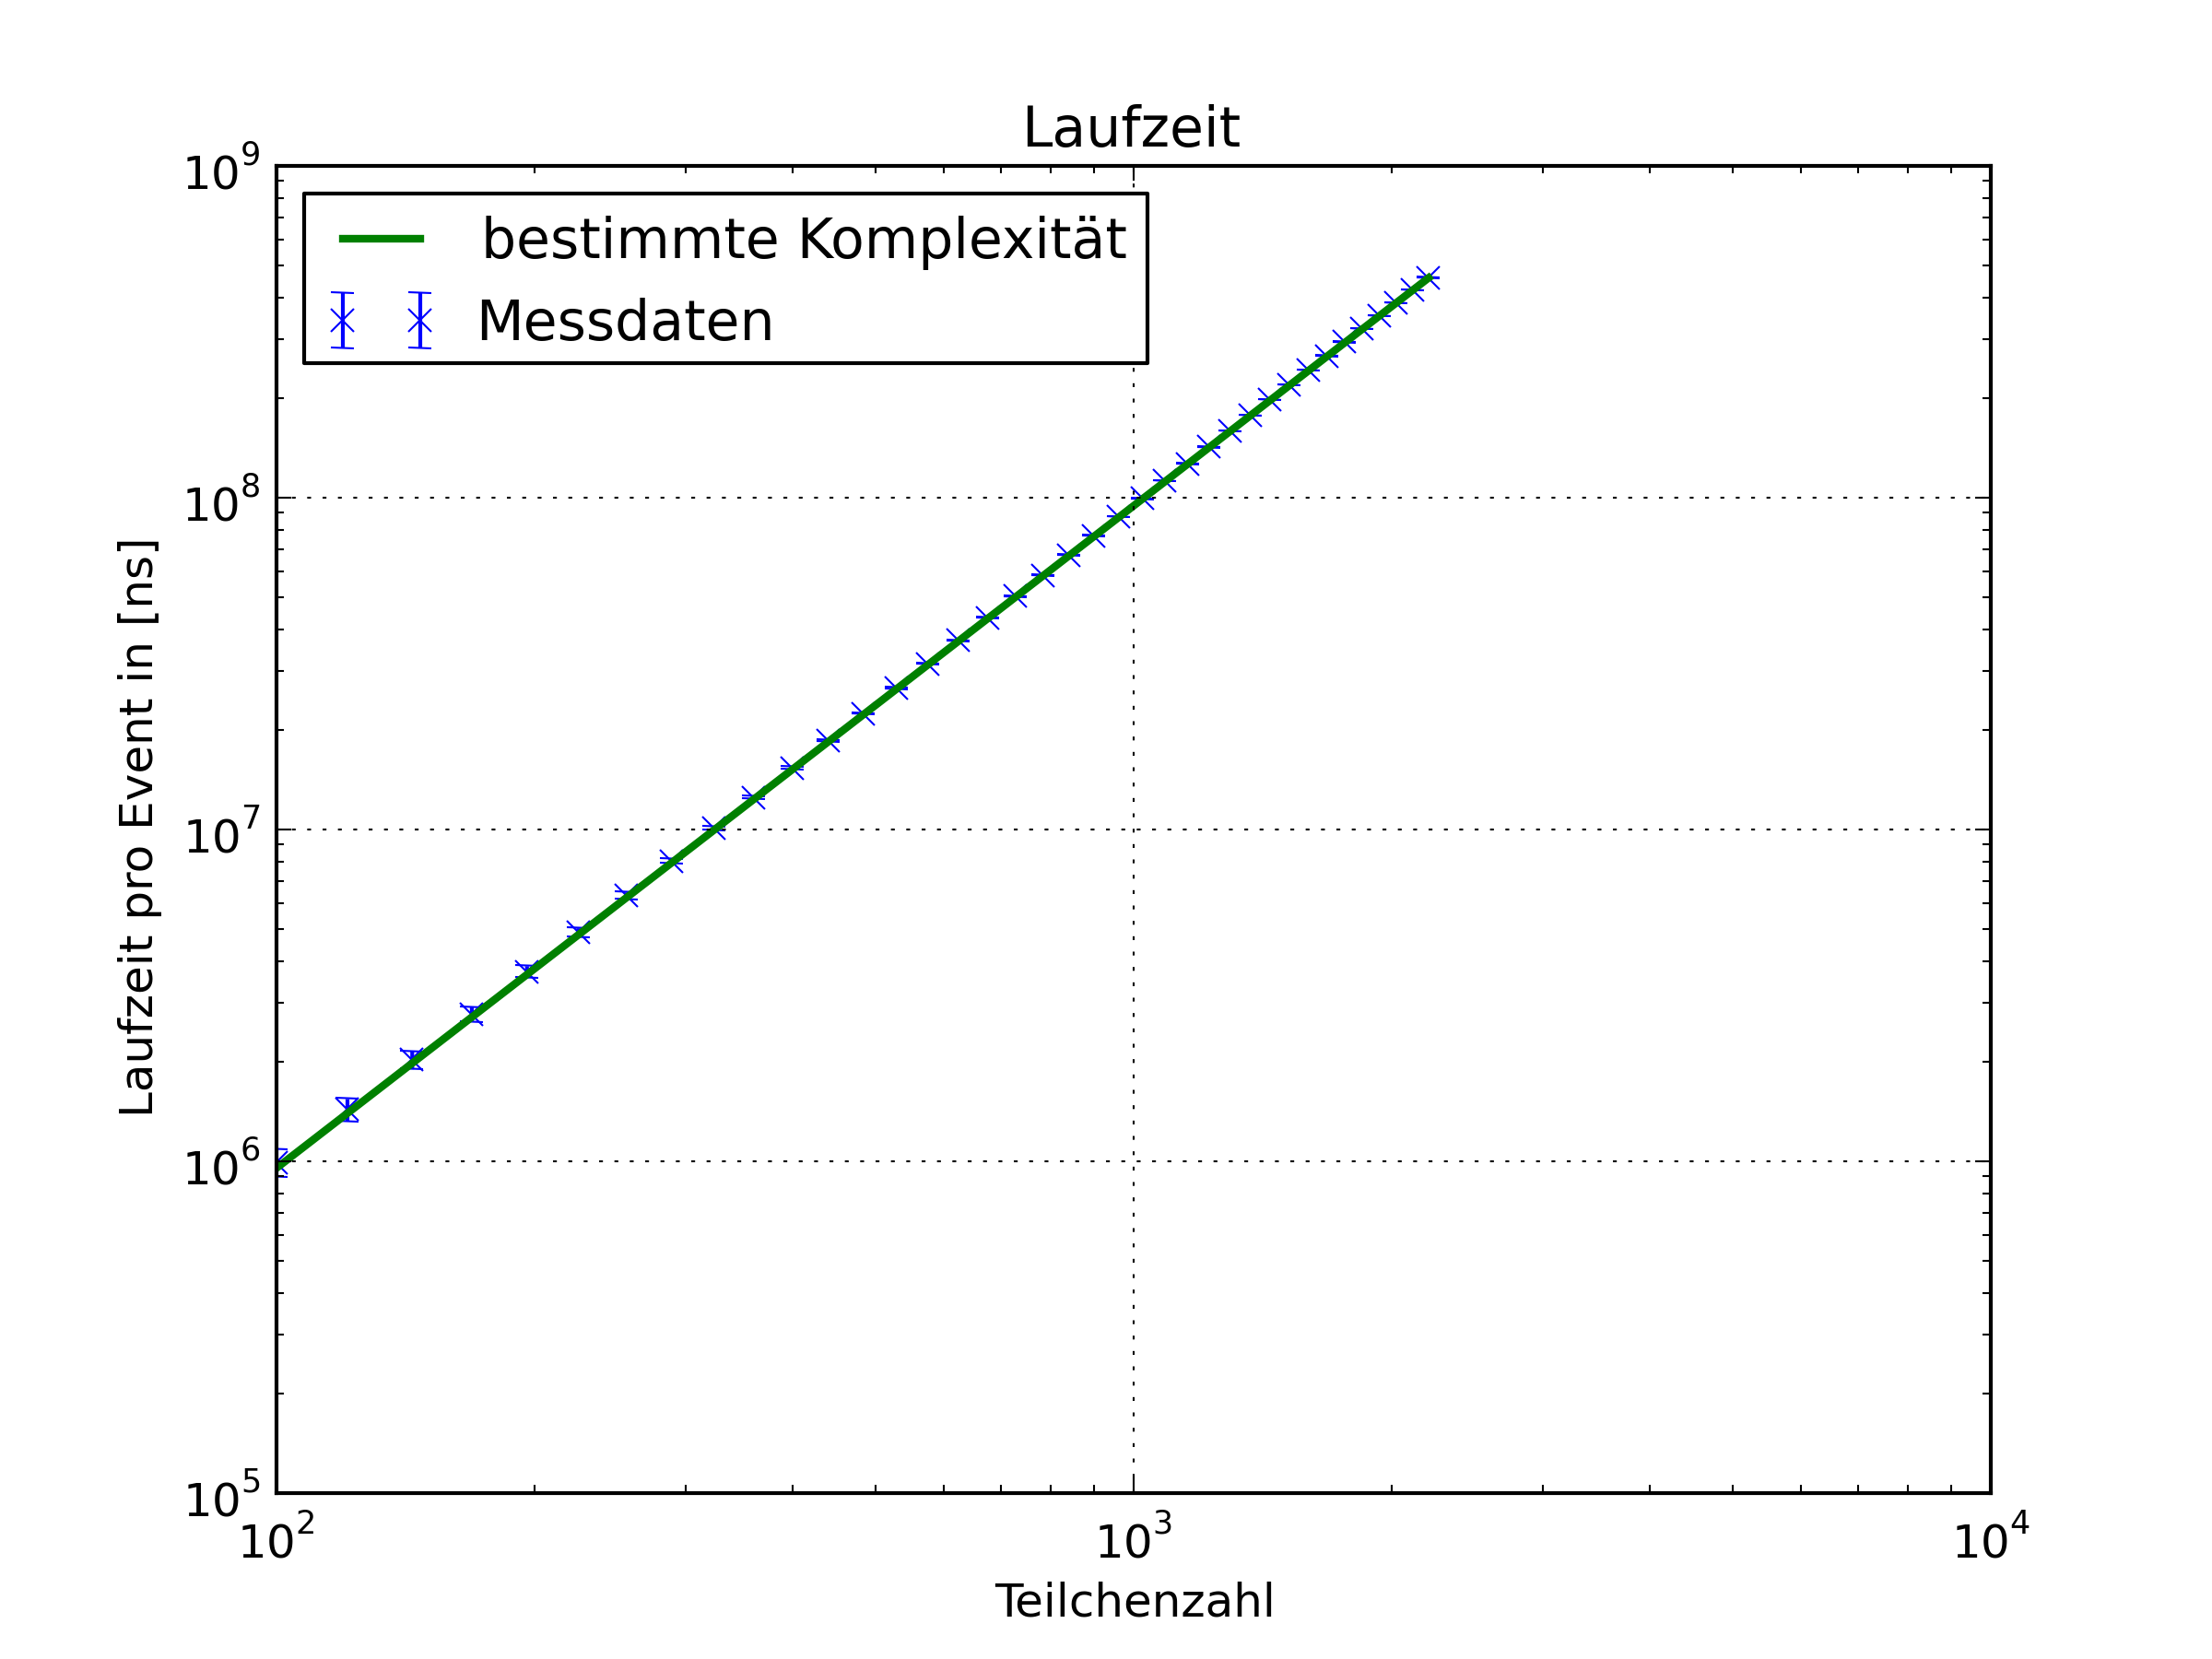
\includegraphics[width=0.80\textwidth]{img/A1_runtime.png}
	\caption{Laufzeit der einfachen Event-Driven Molekulardynamik-Simulation. Die ermittelte Komplexit�t betr�gt $O(N^2.00)$. Dies ist f�r eine ernsthafte wissenschaftliche Simulation unbrauchbar.}
	\label{fig:A1_runtime}
\end{figure}

Um die Komplexit�t zu verringern werden wie schon bei der Molekulardynamik von weichen Teilchen periodische Randbedingungen und eine Zellunterteilung eingef�hrt (siehe hierzu \cite{rapaport2004} und \cite{eibl2012}). Weiterhin wird ein sogenannter Event-Kalender verwendet. Dieser speichert alle berechneten Ereignisse und stellt sie im n�chsten Zeitschritt wieder zur Verf�gung. Somit m�ssen nicht jedes Mal alle Ereignisse neu berechnet werden, was redundante Rechenarbeit spart. Im Endeffekt m�ssen nur diejenigen Ereignisse neu berechnet werden, die durch das ausgewertete Ereignis ung�ltig werden, z.B. zuk�nftige Teilchekollisionen eines gerade sto�enden Teilchens. Die Struktur des Event-Kalenders muss deswegen leistungsf�hig im Bezug auf L�schen und Einf�gen neuer Ereignisse sein. In dieser Arbeit wurde die Konstruktion des Event-Kalenders von Rapaport verwendet. \cite{rapaport2004} Die Komplexit�t des Programms sollte sich damit theoretisch auf $O(N^1)$ reduzieren. Praktisch lies sich dieser Wert durch Ungenauigkeiten bei der Zeitmessung nicht ganz korrekt beobachten (\fref{fig:A2_runtime}). Eine Komplexit�t von $1.12$ zeigt aber eine deutliche Richtung und ist wesentlich besser als die Komplexit�t ohne Optimierungen.

\begin{figure}[h!]
	\centering
		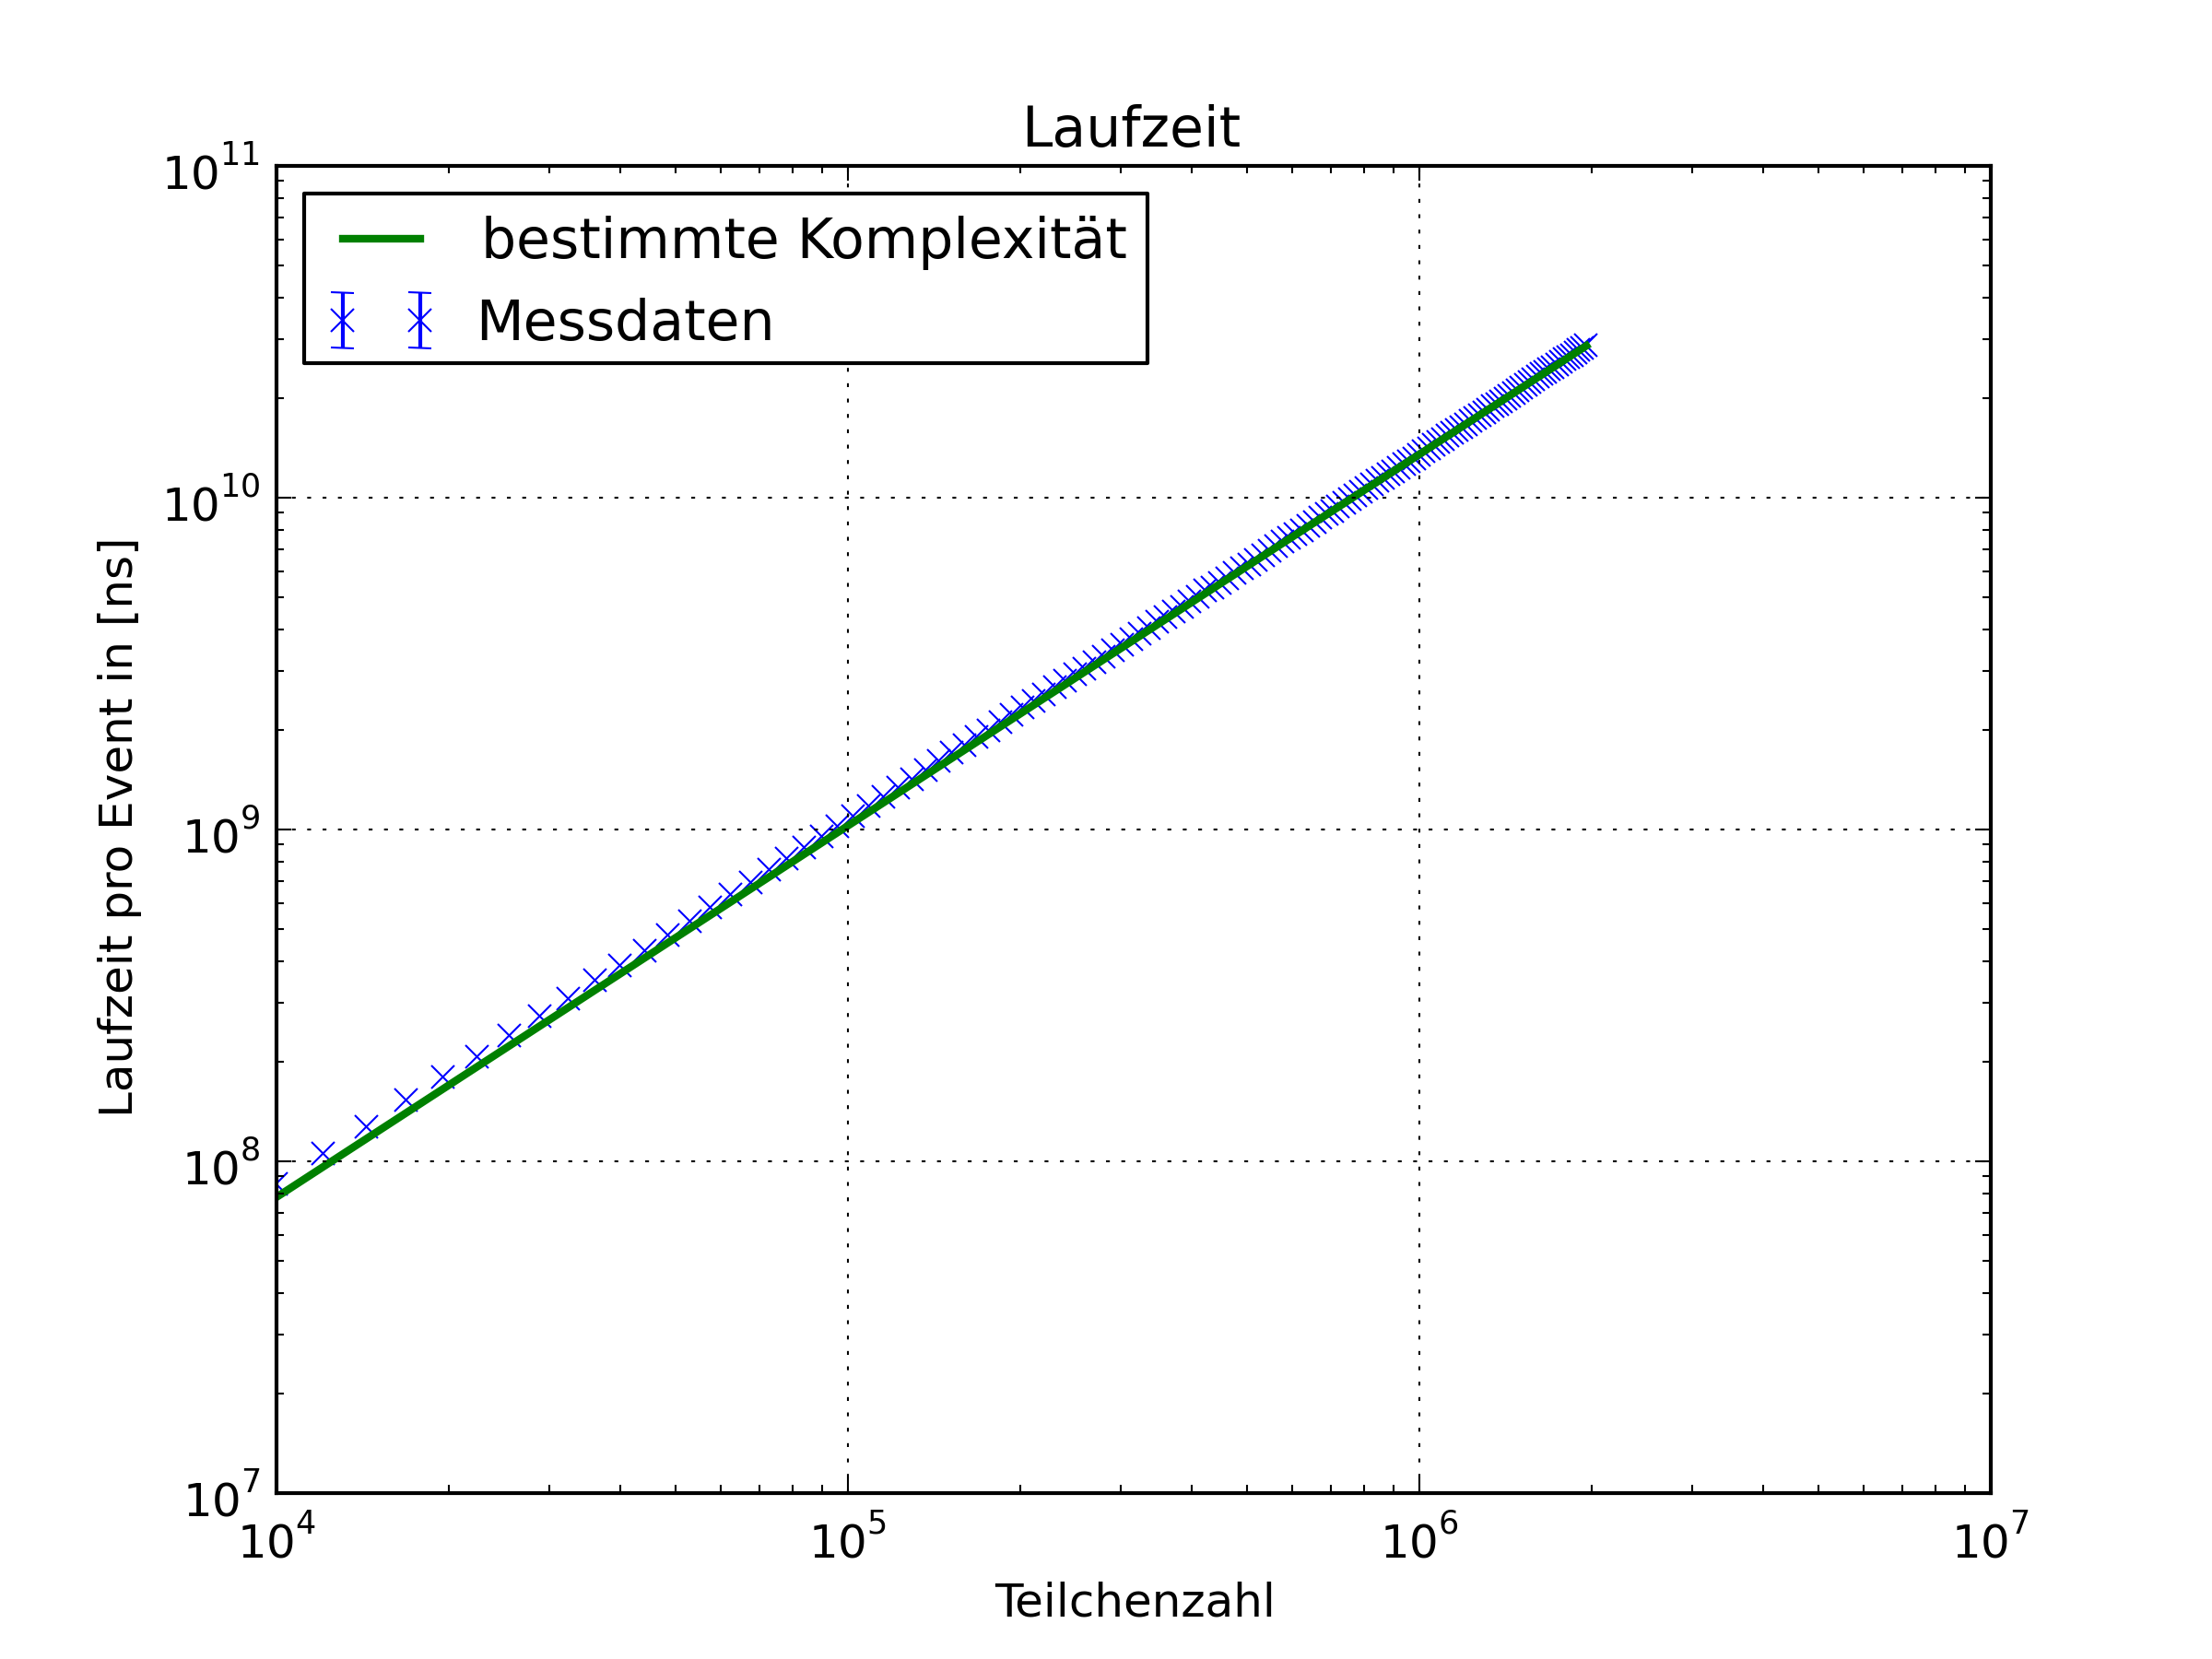
\includegraphics[width=0.80\textwidth]{img/A2_runtime.png}
	\caption{Laufzeit der verbesserten Event-Driven Molekulardynamik-Simulation mit Zellunterteilung und einem Event-Kalender. Die ermittelte Komplexit�t betr�gt $O(N^{1.12})$. Die Abweichung von der theoretisch Erwarteten Komplexit�t von $N^1$, l�sst sich durch eine schwierige Bestimmung der restlichen Last auf dem Computer erkl�ren.}
	\label{fig:A2_runtime}
\end{figure}

